%--------------------------------------------------------------------
\medskip
\section{Mapa}
Todo lo referente a esta sección, se encuentra dentro del paquete \texttt{com.mygdx.iadevproject.map} del proyecto. El mapa que se ha diseñado para este proyecto se muestra en la Figura \ref{mapa:mapa}.
\begin{figure}[!th]
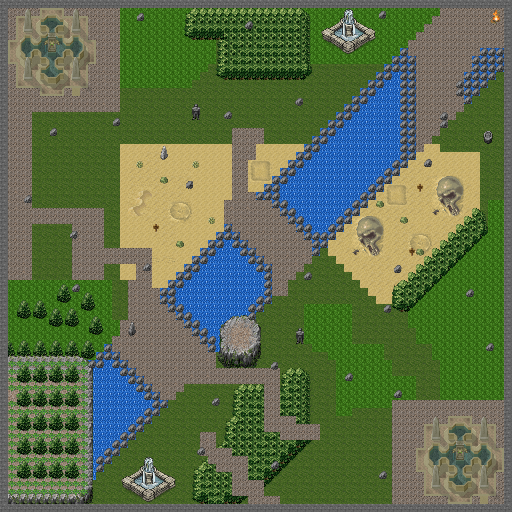
\includegraphics[scale=0.6]{map}
\centering
\caption{Mapa diseñado para el proyecto.}
\label{mapa:mapa}
\end{figure}

Como se puede observar, existen seis tipos de terrenos:
\begin{itemize}
 \item \textbf{Agua y montañas}. Representan los terrenos infranqueables. Como indica el enunciado del proyecto, los dos países se encuentran separados por un río con tres puentes para cruzarlo.
 \item \textbf{Desierto y bosque}. Se identifican de manera directa en el mapa. También se tiene como bosque los árboles que se encuentran dentro la pradera situada en la parte inferior izquierda del mapa.
 \item \textbf{Pradera}. Se corresponde con los tramos de color verde más claro.
 \item \textbf{Sendero}. Se corresponde con el fondo del mapa.
 \item \textbf{Camino}. Se corresponde con los tramos de color gris. Las bases de los países se encuentran encima de este tipo de terreno.
\end{itemize}

Para representar los terrenos en el proyecto, se ha implementado el enumerado \texttt{Ground} que proporciona los siguientes métodos:
\begin{itemize}
 \item \texttt{getCost()}. Debido a que cada terreno tiene un coste asociado, este método devuelve dicho coste.
 \item \texttt{getGround(int cost)}. Se trata de un método estático que dado un coste, devuelve el terreno al que pertenece. Si el coste que se pasa como argumento no se corresponde con ningún terreno, devuelve \texttt{null}.
\end{itemize}

También podemos observar que cada uno de los equipos tiene un manantial donde los personajes pueden curarse y a donde van cuando estos mueren. \\

Para diseñar el mapa, se ha hecho uso de la herramienta \texttt{Tiled Map Editor} \cite{tiledMap} que proporciona una sencilla forma de diseñar mapas por capas, permitiendo que puedas crear capas de distintos tipos (de tiles, de objetos, etc), lo que nos facilita la creación e inicialización de los distintos grids que utilizamos. Lógicamente, las capas que se encuentran en el mapa, se corresponden con los distintos tipos de terrenos mencionados anteriormente (excluyendo la capa de objetos). \\

Para introducir el mapa diseñado en el proyecto, \texttt{LibGDX} nos proporciona la clase \texttt{TiledMap}. Sin embargo, esta clase, a la hora de renderizar, si existe alguna capa de objetos por defecto, no la dibuja. Por este motivo, implementamos la clase \texttt{TiledMapIADeVProject}, que sobreescribe los métodos de renderizado para que se dibujen las capas de objetos. \\

Una vez que tenemos el mapa diseñado e introducido en nuestro proyecto, hay que inicializar los distintos grids en correspondencia con dicho mapa. Para ello, está la clase \texttt{MapsCreatorIADeVProject}, que proporciona un único método estático \texttt{createMaps()} y que se encarga de recorrer, para cada terreno, su capa correspondiente e inicializar los grids a los valores correspondientes.


























